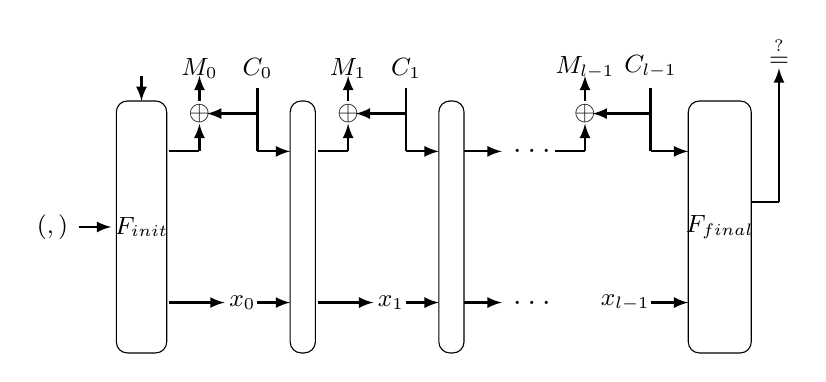
\begin{tikzpicture}[scale=0.32]

\tikzset{SpongePerm/.style=rounded corners=4pt,};

%% 
\begin{scope}[xshift=0cm]


\draw[->,>=latex,thick] (0,5) node[left] {  \small $(\key,\nonce)$} -- ++ (1.3,0);
\draw[->,>=latex,thick] (2.5,11) node[above] {\small$\associateddata$} -- ++ (0,-1);

\draw[SpongePerm] 
    	(1.5,0) rectangle node { \small $F_{init}$} ++(2,10);
 
\end{scope}

\begin{scope}[xshift=0.2cm]



\begin{scope}[xshift = 5.9cm]

\foreach \z in {0,1} {
\begin{scope}[xshift=\z*5.9cm]

\draw[thick]  (-2.5,8) --++ (1.2,0)  ;
\draw[->,>=latex,thick]  (-1.3,8) --++ (0,1.1)  ;
  \node[thick] (xm1) at (-1.3,9.5) {$\oplus$};
\draw[->,>=latex,thick] (-1.3,10) --++ (0,1)  ;
\draw (-1.3,10.5) node[above] { \small $M_{\z}$};
\draw[->,>=latex,thick] (1,9.5) -- (-1,9.5)  ;

\draw[thick] (1,10.5) node[above] { \small $C_{\z}$} -- (1,8);
    
\draw[->,>=latex,thick]  (-2.5,2) -- (-0.3,2)  ;
\draw (0.4,2) node{\small $x_{\z}$};


\draw[SpongePerm] 
    		(2.3,0) rectangle node{\small $\permutation$} ++(1,10);


    \draw[->,>=latex,thick] (1,8) -- ++(1.3,0);
    \draw[->,>=latex,thick] (1,2) -- ++(1.3,0);


  \end{scope}
}

\end{scope}
  %%
  
    \begin{scope}[xshift=15.1cm]
    
    \draw[->,>=latex,thick]  (0,8)--++ (1.5,0)  ;
    \draw[->,>=latex,thick]  (0,2)--++ (1.5,0) ;
        \draw (2.8,8) node {\large \ldots};
    \draw (2.8,2) node {\large \ldots};

  \end{scope}
%%  

\begin{scope}[xshift=20.7cm]

\begin{scope}[xshift=0.5cm]
\draw[thick]  (-2.5,8) --++ (1.2,0)  ;
\draw[->,>=latex,thick]  (-1.3,8) --++ (0,1.1)  ;
  \node[thick] (xm1) at (-1.3,9.5) {$\oplus$};
\draw[->,>=latex,thick] (-1.3,10) --++ (0,1)  ;
\draw (-1.3,10.5) node[above] { \small $M_{l-1}$};
\draw[->,>=latex,thick] (1.3,9.5) -- (-1,9.5)  ;
\end{scope}
    
        %\draw[edge,thick] (-1.5,8) -- ++(1.5,0);
 \draw[thick] (1.8,10.5) node[above] {\small $C_{l-1}$} -- (1.8,8);
%\draw[edge,thick]  (-2.5,2) -- (-0.3,2)  ;
\draw (0.8,2) node{\small $x_{l-1}$};
 
% \fill[red!30] (0,0) rectangle  ++ (1.8,7);
%\draw (0,0) rectangle node{\small $x_{\cipherlength-1}$} ++ (1.8,7);
%\fill[blue!30] (0,7) rectangle  ++ (1.8,3);
%\draw(0,7) rectangle node{\small $\cipherblock$} ++ (1.8,3);
 
  \begin{scope}[xshift=0.8cm]
  \draw[SpongePerm] 
    	(2.5,0) rectangle node {\small $F_{final}$} ++(2.5,10);
     \draw[->,>=latex,thick] (1,8) -- ++(1.5,0);
          \draw[->,>=latex,thick] (1,2) -- ++(1.5,0);
          
     \draw[thick] (5,6) --++ (1.1,0);
    \draw[->,>=latex,thick] (6.1,6) --++ (0,5.3);
   \draw (6.1,11) node[above] {\small $\tagAEAD \stackrel{?}{=} \tagAEAD$};
\end{scope}

       
\end{scope}
  
\end{scope}


\end{tikzpicture}
